\documentclass[12pt,twocolumn]{article}

\usepackage[T1]{fontenc}
\usepackage[utf8]{inputenc}
\usepackage[spanish, mexico,es-noindentfirst]{babel}
\usepackage{graphicx}
\usepackage{amsmath,physics}

\usepackage[
  paper=a3paper,
  top=3mm,
  left=10mm,
  right=10mm,
  bottom=5mm,
  footskip=7mm,
  includefoot
]{geometry}

\usepackage{xcolor}

\usepackage[
  colorlinks=true,
  linkcolor={blue!60!black},
  citecolor={green!50!black},
  urlcolor={magenta!70!black},
  filecolor={magenta!70!black},
  pdfborder={0 0 0},
  breaklinks=true
]{hyperref}


\usepackage{listings}
\usepackage{minted}

\setminted[fortran]{
    style=emacs,
    linenos=true,
    fontsize=\scriptsize,
    breaklines=true,
    frame=lines,
    framesep=2mm,
    numbersep=2pt,        
    xleftmargin=12pt      
}
\pagestyle{plain}
\usepackage{ragged2e}



\usepackage{csquotes}
\usepackage[
  backend=biber,
  bibstyle=apa,
  citestyle=numeric-comp,
  sorting=ynt,
  maxnames=3,minnames=1
]{biblatex}

\makeatletter
\RequireBibliographyStyle{numeric}
\makeatother

\addbibresource{refs.bib}

% --- % --- % --- % --- % --- % --- % --- % --- % --- 
\newcommand{\mititulo}{Solución numérica a la ecuación de calor en dos dimensiones utilizando fortran}
\newcommand{\misubtitulo}{Informe del curso ``Temas Selectos de Alto Rendimiento''}
\newcommand{\miautor}{Jesús Omar Franco Franco}
\newcommand{\mifecha}{viernes 5 de junio de 2026}

\begin{document}

\twocolumn[{%
  \begin{center}
    \noindent
    \begin{minipage}[c]{0.18\textwidth}
      \centering
      
\includegraphics[width=\linewidth]{logo_if.png}
    \end{minipage}%
    \hfill
    \begin{minipage}[c]{0.60\textwidth}
      \centering
      {\Large\bfseries \mititulo \par}
      \vspace{0.4em}
      {\large \misubtitulo \par}
      \vspace{0.6em}
      {\large \miautor \par}
      \vspace{0.3em}
      {\normalsize \mifecha \par}
    \end{minipage}%
    \hfill
    \begin{minipage}[c]{0.18\textwidth}
      \centering
      
\includegraphics[width=\linewidth]{logo_unam.png}
    \end{minipage}

    \vspace{1em}
    \hrule
    \vspace{1.2em}

    % --- Abstract ---
    \begin{minipage}{0.85\textwidth}
      \justify
      {\small Este curso se enfocó en paralelización con openmp y openacc y fue impartido por el profesor Juan Carlos Cajas García (¡gracias profesor!)}.
      \begin{abstract}
      {\it
        En este informe se explica el funcionamiento del código \texttt{calor2D.f90}, el cual calcula numéricamente la solución estacionaria de la ecuación de calor con condiciones de frontera de Dirichlet. El caso de una dimensión (1D) sólo puede llevarse a cabo de forma secuencial usando un método de solución exacta a la discretización de la ecuación de difusión en 1D conocido como \emph{el algoritmo de Thomas}, mientras que para 2D se utilizó nuevamente dicho algoritmo en una rutina para ejecutarlo de forma paralelizada usando \texttt{openmp} repartiéndolo en las diferentes líneas en las direcciones $x$ y $y$. Este informe se enfoca en comprender el algoritmo, su implementación en Fortran usando openmp así como los resultados y el rendimiento obtenido mediante la paralelización utilizando diferentes números de hilos simultáneamente.
        }
      \end{abstract}
    \end{minipage}
    \vspace{1.5em}
  \end{center}
}]

\tableofcontents
\section{Introducción}

La ecuación de difusión de calor 
$$\pdv{T}{t}=D\nabla^2T$$
es un ejemplo paradigmático de un modelo físico sencillo. Poder resolverlo numéricamente es un buen antecedente para poder manejar las herramientas necesarias para hacer simulaciones de fenómenos físicos más complicados; por ejemplo, para implementar un método numérico de solución a las ecuaciones de Navier-Stokes, la cual, ha encontrado infinitas aplicaciones en varias disciplinas.

En este texto se exploran los casos de 1 y 2 dimensiones resolviendo únicamente la solución estacionaria. Es decir, imponiendo la ecuación de Laplace
$$\nabla^2T = 0.$$


% --- % --- % --- % --- % --- % --- % --- % --- % --- 
% --- % --- % --- % --- % --- % --- % --- % --- % --- 

\section{Caso 1D}

% --- % --- % --- % --- % --- % --- % --- % --- % --- 
\subsection{Discretización}
En régimen estacionario y sin fuentes, la ecuación de calor en una dimensión se reduce a resolver la ecuación diferencial $T''(x) = 0$ sobre el intervalo $[0,L]$, con condiciones de
Dirichlet $T(0)=T_0$ y $T(L)=T_L$.

Discretizando el dominio en $N$ nodos con espaciamiento $\Delta x = L/(N-1)$
y aproximando la segunda derivada por su diferencia centrada
$$
\dv[2]{T}{x}\approx\frac{T_{i+1}-2T_i+T_{i-1}}{\Delta x^2}.
$$
se obtiene que cada nodo interior queda ligado únicamente a sus vecinos inmediatos
\begin{equation}
\frac{T_{i+1}-2T_i+T_{i-1}}{(\Delta x)^2}=0,\qquad i=1,\dots,N-2.
\label{eq:disc}
\end{equation}
Multiplicando por $(\Delta x)^2$, la ecuación se simplifica a
\begin{equation}
T_{i-1}-2T_i+T_{i+1}=0,\qquad i=1,\dots,N-2.
\label{eq:disc-simp}
\end{equation}

Reuniendo \eqref{eq:disc} con las dos filas referentes a las condiciones de frontera, el problema se
convierte en un sistema lineal $A\,\mathbf{T}=\mathbf{d}$ cuya matriz es
\emph{tridiagonal}: solo son no nulas la diagonal principal $b_i$ y las dos
adyacentes $a_i$ (inferior) y $c_i$ (superior),
\begin{equation}
\begin{pmatrix}
b_0 & c_0 & & \\
a_1 & b_1 & c_1 & \\
& \ddots & \ddots & \ddots \\
& & a_{N-1} & b_{N-1}
\end{pmatrix}
\mathbf{T}=\mathbf{d},
\label{eq:tridiag}
\end{equation}
donde $a_i=c_i=1$, $b_i=-2$ y $d_i=0$ para $1\leq i < N-1$.
Para las condiciones de Dirichlet en ambos puntos de la frontera $b_0=b_{N-1}=1$, $a_0=a_{N-1}=0$, $d_0=T_0$ y $d_{N-1}=T_L$.

Como curiosidad, si se deseara implementar una condición de Neumann (por una derivada conocida $T'(0) = q$ en el lado izquierdo), basta utilizar una diferencia hacia adelante $\dfrac{T_1 - T_0}{\Delta x} = q$. Al reacomodar multiplicando por $\Delta x$ se llega a la forma $-T_0 + T_1 = q \Delta x$, con lo cual se asignarían libremente los componentes de la matriz a $b_0=-1$, $c_0=1$ y $d_0=q\Delta x$.

% --- % --- % --- % --- % --- % --- % --- % --- % --- 
\subsection{El algoritmo de Thomas}
La estructura diagonal de la matriz en \eqref{eq:tridiag}  permite resolver el sistema de ecuaciones sin una eliminación
gaussiana completa. El algoritmo de Thomas lo hace en dos barridos. En el
barrido hacia adelante se eliminan los coeficientes inferiores (partiendo de
$c_0'=c_0/b_0$ y $d_0'=d_0/b_0$),
$$
c_i'=\frac{c_i}{b_i-a_i c_{i-1}'},\qquad
d_i'=\frac{d_i-a_i d_{i-1}'}{b_i-a_i c_{i-1}'},
$$
y en la sustitución hacia atrás se recupera la solución,
$$
T_{N-1}=d_{N-1}',\qquad T_i=d_i'-c_i'\,T_{i+1}.
$$
Su costo es $O(N)$, frente al $O(N^3)$ de una eliminación general, lo que hace
de Thomas el método natural para la matriz tridiagonal que produce el esquema
de diferencias finitas en 1D%
\footnote{%
Se puede consultar una explicación más completa de este algoritmo y su pseudocódigo en la página de wikipedia
\href{https://en.wikipedia.org/wiki/Tridiagonal_matrix_algorithm}{Tridiagonal matrix algorithm}.
}
.
% --- % --- % --- % --- % --- % --- % --- % --- % --- 
\subsection[%
El programa \texorpdfstring{\texttt{calor1D.f90}}{calor1D.f90} y el módulo \texorpdfstring{\texttt{tridiagonal.f90}}{tridiagonal.f90} 
]{%
El programa \texorpdfstring{\texttt{calor1D.f90}}{calor1D.f90} secuencial y el módulo \texorpdfstring{\texttt{tridiagonal.f90}}{tridiagonal.f90} 
}

El módulo \texttt{tridiagonal.f90} contiene una implementación del algoritmo de Thomas en Fortran. Este méto, como se mencionó en el apartado anterior, aprovecha que la matriz del problema solo tiene elementos distintos de cero en la diagonal principal y sus diagonales vecinas. Primero elimina los términos inferiores de la matriz y después calcula la solución mediante sustitución hacia atrás, obteniendo el perfil de temperatura de manera rápida y eficiente.

\inputminted{fortran}{tridiagonal.f90}

El código \texttt{calor1D.f90} simplemente construye los arreglos 1D para el sistema. Cabe notar que establece las condiciones de frontera de la siguiente manera: del lado izquierdo impone una derivada igual a $-1$, y del lado derecho fija $T_L = 0$. Una vez preparado, llama a la subrutina en \texttt{tridiagonal.f90} para resolver todo secuencialmente con el algoritmo de Thomas.
\inputminted{fortran}{calor1D.f90}
Para compilar estos dos códigos y ejecutar el programa se pueden correr en la terminal los siguientes comandos
\begin{minted}[
    breaklines
]{bash}
gfortran tridiagonal.f90 calor1D.f90  -o calor1D
./calor1D
\end{minted}
y el resultado obtenido al ejecutar el programa \verb|calor1D| es la impresión de cada punto en la malla guardado en \verb|xx(-)| y su respectivo valor de temperatura que fue calculado y almacenado en \verb|tt(-)|. En este caso, si se grafican los valores, se obtiene una línea recta con pendiente $T'(x)\equiv-1$ y tal que $T(x=10.0)=0$ (por lo tanto $T(x=0)=10.0$ salvo que con pequeños errores debido a la aritmética de punto flotante).
% --- % --- % --- % --- % --- % --- % --- % --- % --- 
% --- % --- % --- % --- % --- % --- % --- % --- % --- 
\section{Caso 2D}



% --- % --- % --- % --- % --- % --- % --- % --- % --- 
\subsection{Discretización}

En dos dimensiones, la ecuación de Laplace es
$$
\frac{\partial^2 T}{\partial x^2} + \frac{\partial^2 T}{\partial y^2} = 0,
$$
sobre un dominio rectangular $[0,L_x]\times[0,L_y]$ con condiciones de Dirichlet en todas las fronteras. Discretizando con $N_x$ nodos en $x$ y $N_y$ nodos en $y$, con espaciamientos $\Delta x = L_x/N_x$ y $\Delta y = L_y/N_y$, y aproximando cada segunda derivada por diferencias centradas, la ecuación evaluada en el nodo interior $(i,j)$ queda
\begin{equation}
  \frac{T_{i-1,j} - 2T_{i,j} + T_{i+1,j}}{(\Delta x)^2}
  +\frac{T_{i,j-1} - 2T_{i,j} + T_{i,j+1}}{(\Delta y)^2} = 0.
  \label{eq:disc2d}
\end{equation}

A diferencia del caso 1D, aquí los nodos en $x$ están acoplados con los de $y$, por lo que el sistema resultante ya no es tridiagonal en el sentido estricto: es un sistema disperso de $N_x N_y$ incógnitas que no puede resolverse directamente con el algoritmo de Thomas.

\subsubsection*{Método de líneas (ADI simplificado)}

Para conservar la eficiencia del algoritmo de Thomas, se recurre a un método iterativo por \emph{barridos alternos de líneas}. La idea es fijar temporalmente una dirección y resolver la otra como un sistema tridiagonal 1D. Partiendo de \eqref{eq:disc2d} y reagrupando,

\begin{itemize}
  \item \textbf{Barrido en $x$}: para cada fila $j$ fija, los valores $T_{i,j\pm1}$ se tratan como conocidos y se pasan al lado derecho. La ecuación en el nodo $(i,j)$ adopta la forma
  \begin{multline}
    -\frac{T_{i,j-1}+T_{i,j+1}}{(\Delta y)^2}
    =
    \frac{1}{(\Delta x)^2}\,T_{i-1,j}
    - 2\!\left(\frac{1}{(\Delta x)^2}+\frac{1}{(\Delta y)^2}\right)T_{i,j}
    \\+ \frac{1}{(\Delta x)^2}\,T_{i+1,j},
    \label{eq:sweepx}
  \end{multline}
  que es un sistema tridiagonal de tamaño $N_x$ por cada $j$.

  \item \textbf{Barrido en $y$}: para cada columna $i$ fija, los valores $T_{i\pm1,j}$ se tratan como conocidos y se pasan al lado derecho. La ecuación en $(i,j)$ es
  \begin{multline}
     -\frac{T_{i-1,j}+T_{i+1,j}}{(\Delta x)^2}
    =
    \frac{1}{(\Delta y)^2}\,T_{i,j-1}
    - 2\!\left(\frac{1}{(\Delta x)^2}+\frac{1}{(\Delta y)^2}\right)T_{i,j}
    \\+ \frac{1}{(\Delta y)^2}\,T_{i,j+1},
    \label{eq:sweepy}
  \end{multline}
  que es un sistema tridiagonal de tamaño $N_y$ por cada $i$.
\end{itemize}


% --- % --- % --- % --- % --- % --- % --- % --- % --- 
\subsection{Convergencia}

Una condición de convergencia se puede implementar en los dos barridos mencionados en el apartado anterior si se repiten iterativamente hasta que la norma euclidiana de la diferencia entre iteraciones sucesivas cae por debajo de una tolerancia $\varepsilon$,
$$
  \left\|T^{(k+1)} - T^{(k)}\right\|_2 < \varepsilon.
$$
Cada uno de los sistemas tridiagonales se resuelve con el algoritmo de Thomas.

% --- % --- % --- % --- % --- % --- % --- % --- % --- 
\subsection{OpenMP}
OpenMP (Open Multi-Processing) es una interfaz de programación de aplicaciones (API) diseñada para el desarrollo de software en paralelo en arquitecturas de memoria compartida, compatible con los lenguajes C, C++ y Fortran (en nuestro curso, vimos únicamente cómo usarlo en Fortran). El modelo de ejecución se basa en una estructura secuencial-paralela en la que el programa inicia con un único hilo conductor, denominado hilo maestro. Al alcanzar una región identificada como paralela, dicho hilo genera un conjunto de hilos de soporte que ejecutan las tareas simultáneamente, integrándose nuevamente al hilo principal una vez concluida la operación.

La principal ventaja de OpenMP radica en su capacidad para abstraer la complejidad de bajo nivel en la gestión de hilos, permitiendo implementar paralelismo mediante directivas de compilador sencillas (conocidas como \textit{pragmas}), tales como \texttt{!\$omp parallel do}. Asimismo, el sistema ofrece mecanismos precisos para delimitar el alcance de las variables en ámbitos públicos o privados, garantizando así un control eficiente sobre las condiciones de carrera y la sincronización. Para su implementación, se requiere la inclusión de la librería de cabecera \texttt{omp.h} y la activación de la bandera \texttt{-fopenmp} durante el proceso de compilación\footnote{%
Para una introducción amena a OpenMP se recomienda consultar la referencia \cite{ltoma_openmp}.
}.




% --- % --- % --- % --- % --- % --- % --- % --- % --- 
\subsection[%
El programa \texorpdfstring{\texttt{calor2D.f90}}{calor2D.f90}
]{%
El programa \texorpdfstring{\texttt{calor2D.f90}}{calor2D.f90} paralelizado con openmp
}
A continuación presentamos y explicamos el código en el que se implementa la discretización y la condición de paro que se explicó anteriormente. En el apéndice \ref{sec:apendiceA} se colocó el código del módulo \texttt{utiles}, escrito en el programa \texttt{mod\_utiles.f90}, en el cual se especifica el número de nodos en cada dirección ($N_x=120,N_y=60$) y el máximo de iteraciones permitidas ($1000$ iteraciones).

\inputminted{fortran}{calor2D_paralelo.f90}
En la línea 3 se añade \texttt{use omp\_lib}, lo que permite al programa acceder a las funciones y directivas de OpenMP.

En las líneas 76 a 83 y 87 a 90 se inicializan las condiciones de frontera. Como se menciona en los comentarios del código, estos bucles no se paralelizan debido a que el volumen de trabajo es mínimo; el costo computacional (\emph{overhead}) de crear y gestionar los hilos superaría el beneficio de la ejecución paralela en un arreglo tan pequeño.

\subsubsection*{Sincronización en la actualización del estado (Líneas 95--101)}

Al inicio de cada paso en el bucle temporal, se realiza una copia del estado actual de la temperatura al arreglo de la iteración anterior (\texttt{tt(:,:,2)}). Esto se paraleliza mediante la directiva \texttt{!\$omp parallel do}. Dado que no existen dependencias de datos entre celdas distintas para esta operación de asignación, los hilos de ejecución distribuyen las filas de la matriz de manera independiente y segura.

\subsubsection*{Barridos de líneas y alcance de variables (Líneas 109--153 y 161--202)}

En la línea~3 se añade \texttt{use omp\_lib} para dar acceso a las funciones de OpenMP.

Las líneas~76--83 y~87--90 inicializan las condiciones de frontera sin paralelismo,
ya que el arreglo es tan pequeño que el costo de gestionar los hilos superaría cualquier ganancia.

\subsubsection*{Copia del estado anterior (Líneas 95--101)}

Al inicio de cada paso temporal se copia la temperatura actual al arreglo \texttt{tt(:,:,2)}.
Esta operación no tiene dependencias entre celdas, así que se paraleliza con
\texttt{!\$omp parallel do} y cada hilo trabaja sobre una porción de filas de forma independiente.

\subsubsection*{Barridos de líneas (Líneas 109--153 y 161--202)}

Los dos barridos alternos (\texttt{barrido\_y} y \texttt{barrido\_x}) son el núcleo del rendimiento:

\begin{itemize}
    \item \textbf{\texttt{!\$omp parallel do}:} crea la región paralela y reparte el bucle externo entre los hilos.
    \item \textbf{\texttt{default(none)}:} obliga a declarar explícitamente el alcance de cada variable, evitando errores de memoria compartida.
    \item \textbf{Variables compartidas (\texttt{shared}):} las constantes físicas (\texttt{deltax}, \texttt{deltay}), la matriz de temperaturas (\texttt{tt}) y los vectores de frontera (\texttt{cfx}, \texttt{cfy}) son compartidos porque todos los hilos los leen y escriben en regiones bien delimitadas por sus índices.
    \item \textbf{Variables privadas (\texttt{private}):} los arreglos del sistema tridiagonal de cada línea (\texttt{ax}, \texttt{bx}, \texttt{cx}, \texttt{rx}, \texttt{tx} y sus equivalentes en~$y$) son locales a cada hilo. Cada hilo resuelve su propio sistema con la subrutina \texttt{tri} (líneas~142 y~190); si fueran compartidos, los hilos se sobreescribirían entre sí y el resultado sería incorrecto.
\end{itemize}

\subsubsection*{Cálculo del residuo (Líneas 206--215)}

Para verificar convergencia se suma el cuadrado de las diferencias de temperatura entre iteraciones.
Como es una acumulación en una sola variable escalar, se usa \texttt{reduction(+:residuo)}:
cada hilo acumula su parte en una copia privada y OpenMP las combina al final, sin condiciones de carrera.

\subsubsection*{Exportación a VTK (Líneas 229--235)}

La escritura del archivo VTK se hace con un solo hilo, en orden estricto por filas y columnas.
Paralelizarla haría que los hilos escribieran en desorden, corrompiendo el archivo y
haciéndolo ilegible para herramientas como \texttt{gnuplot} o \texttt{ParaView}.

% --- % --- % --- % --- % --- % --- % --- % --- % --- 
\section{Resultados}
Para compilar y ejecutar el programa calor2D se usan los siguientes comandos
\begin{minted}[
    breaklines
]{bash}
gfortran tridiagonal.f90 mod_utiles.f90 calor2D_paralelo.f90 -o calor2D
./calor2D
\end{minted}
\subsection{Solución estacionaria}
Como se mencionó antes, los resultados de la simulación calor2D se guardaron en en un archivo llamado \texttt{salida.vtk}, el cual puede ser visualizado fácilmente usando Paraview.
\begin{figure}[H]
    \centering
    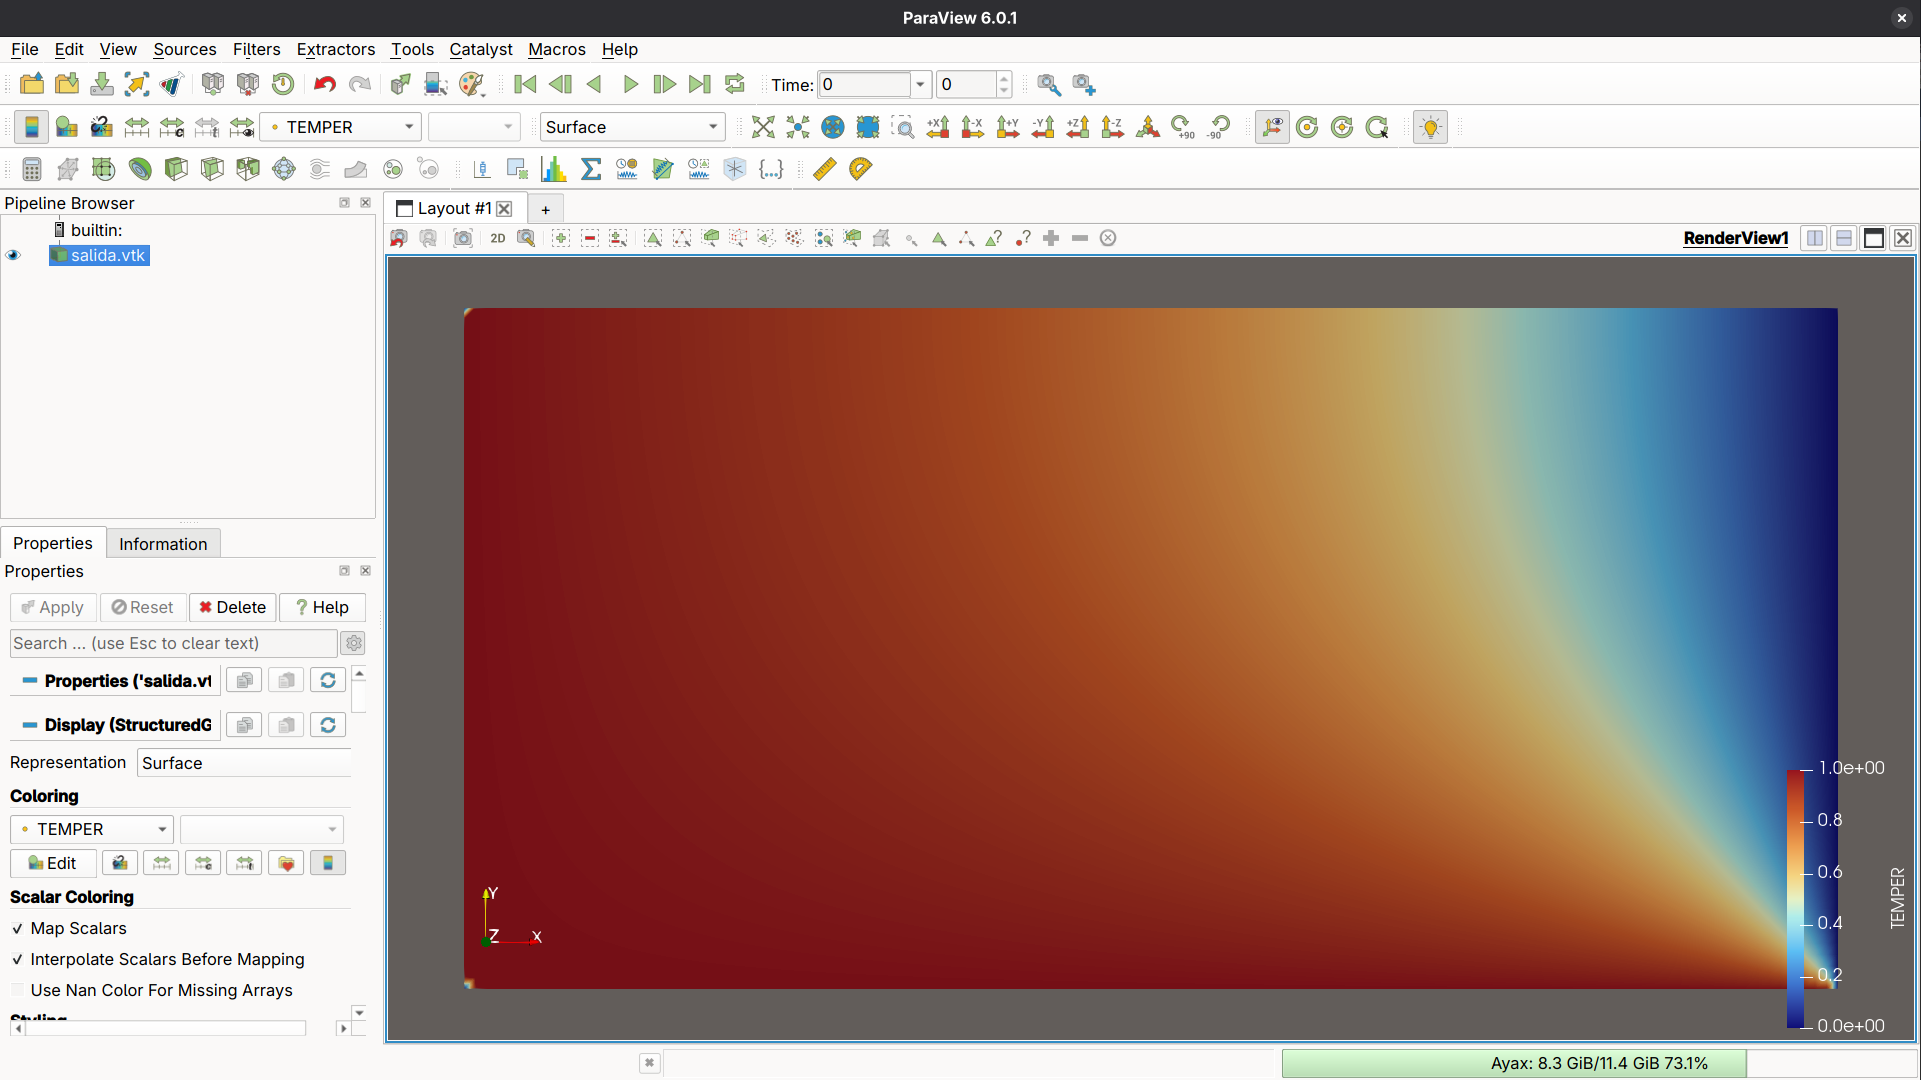
\includegraphics[width=0.98\linewidth]{sol_estacionaria.png}
    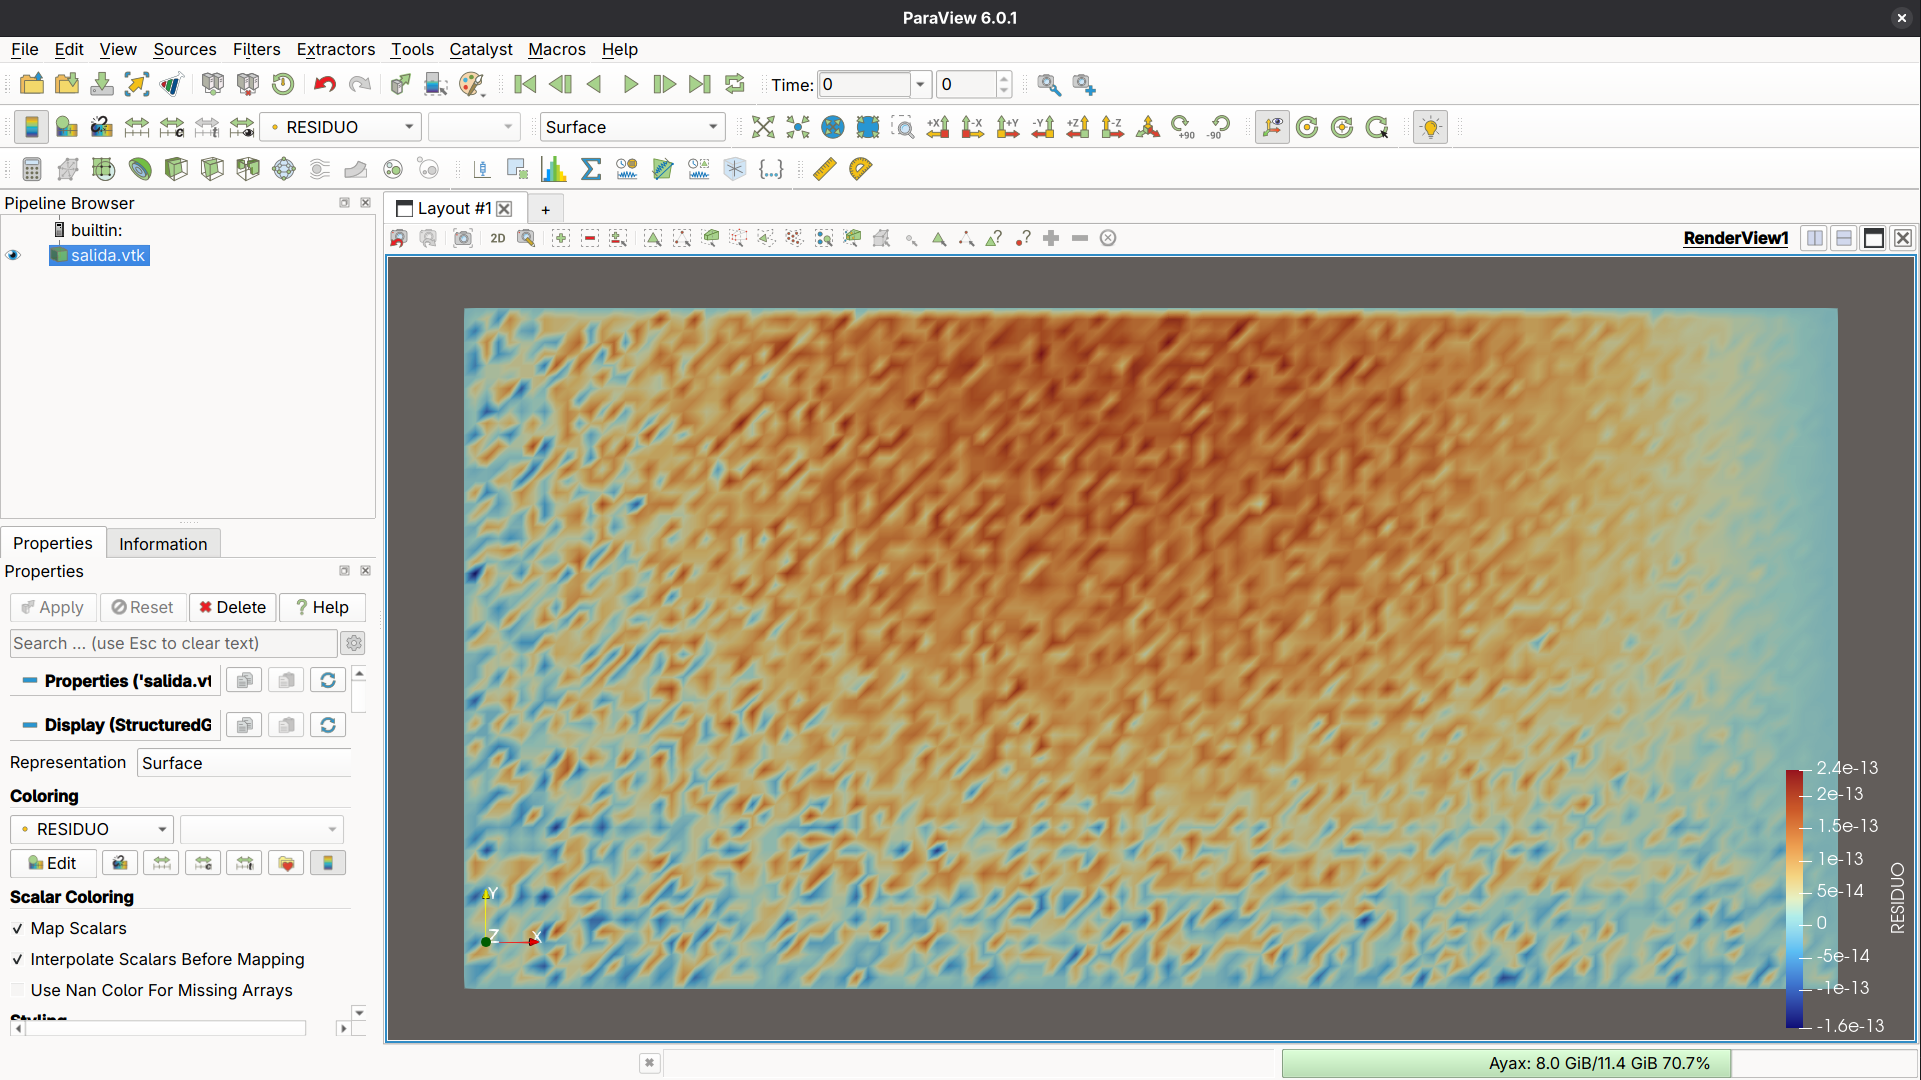
\includegraphics[width=0.98\linewidth]{residuo.png}
    \caption{Gráficas de la solución estacionaria \texttt{tt(:,:)} y su residuo \texttt{resid\_tt(:,:)} usando Paraview obtenidos de ejecutar el programa \texttt{calor2D} y leer el archivo \texttt{salida.vtk}.}
    \label{fig:sol_estacionaria}
\end{figure}
En la figura \ref{fig:sol_estacionaria} se observa claramente que se cumplen las condiciones de frontera establecidas; $+1$ en las fronteras izquierda e inferior, $0$ en la frontera derecha y condición de Neumann en la frontera superior. También se observa que el residuo en cada nodo tiene valores de máximo $2.4\times 10^{-13}$, lo que indica que nuestra solución discreta se acerca mucho a la teórica. 

\subsection{Rendimiento}

\begin{figure}[H]
    \centering
    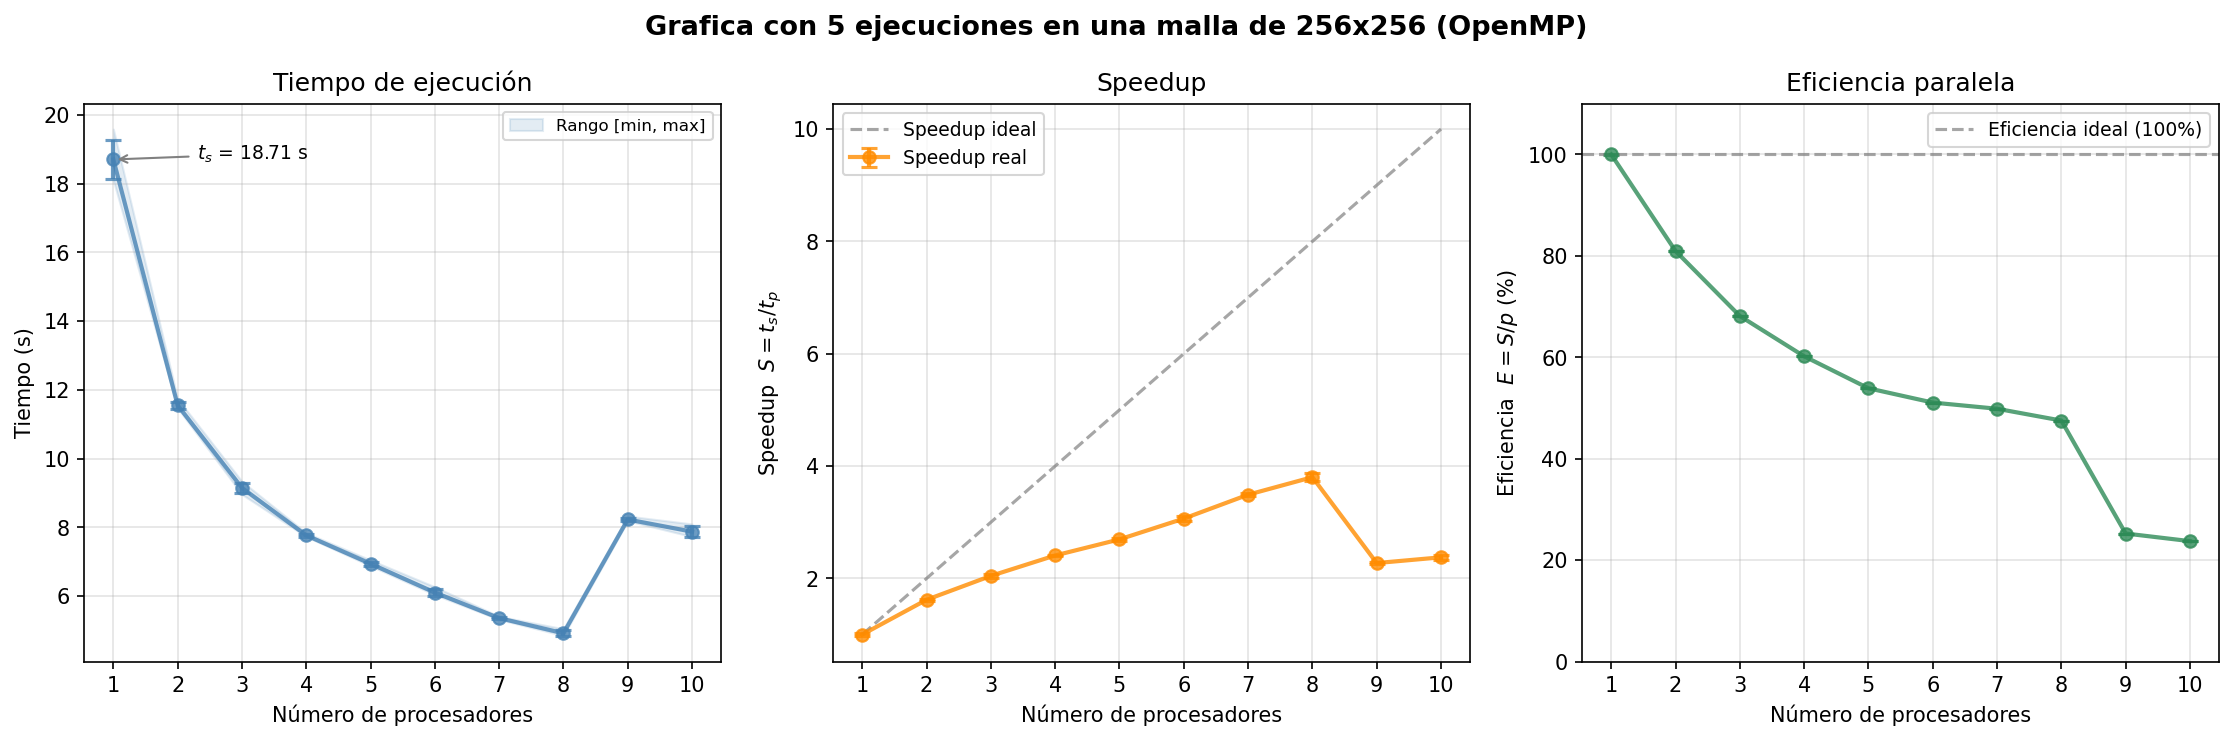
\includegraphics[width=0.99\linewidth]{benchmark_256x256_5_ejecuciones_1a10_hilos.png}
    \caption{Rendimiento obtenido en promedio al ejecutar 5 veces \texttt{calor2D} y medir el tiempo de ejecución.}
    \label{fig:rendimiento}
\end{figure}

La gráfica \ref{fig:rendimiento} analiza el rendimiento de \texttt{calor2D} al aumentar la cantidad de procesadores de uno a diez usando \verb|export OMP_NUM_THREADS|. En ella se observa que la velocidad del cálculo mejora de forma constante a medida que se añaden hilos, pero encuentra su límite óptimo al alcanzar los ocho procesadores (porque es el número de hilos que mi CPU tiene de forma independiente). A partir de este punto, el rendimiento empeora de manera drástica debido a la saturación del sistema.

El análisis del tiempo de ejecución muestra que el programa requiere un máximo de $18.71$ segundos cuando funciona de manera secuencial con un solo procesador. Al incrementar la potencia computacional, el tiempo disminuye progresivamente hasta registrar su punto más rápido con ocho procesadores, donde la tarea se completa en aproximadamente 5 segundos. Sin embargo, al emplear nueve y diez procesadores se eleva el tiempo de ejecución a casi 8 segundos.

La aceleración o \textit{speedup} mide cuántas veces más rápido corre el programa en comparación con su ejecución básica. Aunque la expectativa ideal plantea una aceleración lineal equivalente al número de procesadores utilizados, el comportamiento real muestra que el programa alcanza un tope de velocidad de $3.8$ veces más rápido con ocho procesadores, para luego caer en picada en los casos posteriores. 

Finalmente, la eficiencia paralela refleja el porcentaje de aprovechamiento de cada procesador añadido. Este indicador disminuye desde el segundo procesador y se estabiliza cerca del 50\% entre los cinco y ocho núcleos. Al intentar utilizar nueve y diez procesadores, la eficiencia se desploma al 25\%, lo que demuestra un desperdicio de la capacidad del equipo. Este fenómeno confirma que el procesador físico empleado posee un límite de ocho núcleos, por lo que añadir hilos adicionales genera una congestión que ralentiza el trabajo.

% --- % --- % --- % --- % --- % --- % --- % --- % --- 
\section{Conclusiones}

Se resolvió numéricamente la ecuación de calor estacionaria en 1D y 2D
mediante diferencias finitas. En 1D, la matriz tridiagonal del sistema
permitió aplicar directamente el algoritmo de Thomas que resuelve
el problema de forma exacta (sin considerar el error de la aritmética de punto flotante) y secuencial. En 2D, el acoplamiento entre
direcciones rompe la estructura tridiagonal estricta, pero el método de
barridos alternos de líneas (ADI simplificado) recupera dicha estructura
fila por fila y columna por columna, reaprovechando el mismo algoritmo de
Thomas dentro de un esquema iterativo controlado por una tolerancia
$\varepsilon$.

La paralelización con OpenMP resultó natural: cada línea define un sistema
tridiagonal independiente, por lo que repartir los barridos entre hilos no
introduce dependencias de datos, siempre que los arreglos de cada sistema
se declaren de forma privada (\texttt{private}) y el residuo se acumule con
\texttt{reduction(+:\dots)}.

El análisis de rendimiento confirmó la teoría: el tiempo bajó de
$18.71$\,s en modo secuencial a $\sim5$\,s con ocho hilos, con un
\emph{speedup} máximo de $3.8\times$ y una eficiencia que se estabilizó
cerca del $50\%$. El punto óptimo coincidió exactamente con los ocho
núcleos físicos del CPU; al forzar nueve o diez hilos, la saturación
degradó el desempeño (eficiencia $\sim25\%$). Esto evidencia que la
ganancia paralela está acotada por el \emph{hardware} disponible y que
sobre-suscribir los núcleos es contraproducente.

En conjunto, el trabajo muestra cómo un modelo físico sencillo sirve de
banco de pruebas para combinar un algoritmo clásico eficiente (Thomas) con
paralelismo de memoria compartida.

\printbibliography

\appendix

\section{Programa \texorpdfstring{\texttt{mod\_utiles.f90}}{mod\_utiles.f90}}
\label{sec:apendiceA}
\inputminted{fortran}{mod_utiles.f90}

\end{document}


